\documentclass[english,man]{apa6}

\usepackage{amssymb,amsmath}
\usepackage{ifxetex,ifluatex}
\usepackage{fixltx2e} % provides \textsubscript
\ifnum 0\ifxetex 1\fi\ifluatex 1\fi=0 % if pdftex
  \usepackage[T1]{fontenc}
  \usepackage[utf8]{inputenc}
\else % if luatex or xelatex
  \ifxetex
    \usepackage{mathspec}
    \usepackage{xltxtra,xunicode}
  \else
    \usepackage{fontspec}
  \fi
  \defaultfontfeatures{Mapping=tex-text,Scale=MatchLowercase}
  \newcommand{\euro}{€}
\fi
% use upquote if available, for straight quotes in verbatim environments
\IfFileExists{upquote.sty}{\usepackage{upquote}}{}
% use microtype if available
\IfFileExists{microtype.sty}{\usepackage{microtype}}{}

% Table formatting
\usepackage{longtable, booktabs}
\usepackage{lscape}
% \usepackage[counterclockwise]{rotating}   % Landscape page setup for large tables
\usepackage{multirow}		% Table styling
\usepackage{tabularx}		% Control Column width
\usepackage[flushleft]{threeparttable}	% Allows for three part tables with a specified notes section
\usepackage{threeparttablex}            % Lets threeparttable work with longtable

% Create new environments so endfloat can handle them
% \newenvironment{ltable}
%   {\begin{landscape}\begin{center}\begin{threeparttable}}
%   {\end{threeparttable}\end{center}\end{landscape}}

\newenvironment{lltable}
  {\begin{landscape}\begin{center}\begin{ThreePartTable}}
  {\end{ThreePartTable}\end{center}\end{landscape}}

  \usepackage{ifthen} % Only add declarations when endfloat package is loaded
  \ifthenelse{\equal{\string man}{\string man}}{%
   \DeclareDelayedFloatFlavor{ThreePartTable}{table} % Make endfloat play with longtable
   % \DeclareDelayedFloatFlavor{ltable}{table} % Make endfloat play with lscape
   \DeclareDelayedFloatFlavor{lltable}{table} % Make endfloat play with lscape & longtable
  }{}%



% The following enables adjusting longtable caption width to table width
% Solution found at http://golatex.de/longtable-mit-caption-so-breit-wie-die-tabelle-t15767.html
\makeatletter
\newcommand\LastLTentrywidth{1em}
\newlength\longtablewidth
\setlength{\longtablewidth}{1in}
\newcommand\getlongtablewidth{%
 \begingroup
  \ifcsname LT@\roman{LT@tables}\endcsname
  \global\longtablewidth=0pt
  \renewcommand\LT@entry[2]{\global\advance\longtablewidth by ##2\relax\gdef\LastLTentrywidth{##2}}%
  \@nameuse{LT@\roman{LT@tables}}%
  \fi
\endgroup}


\ifxetex
  \usepackage[setpagesize=false, % page size defined by xetex
              unicode=false, % unicode breaks when used with xetex
              xetex]{hyperref}
\else
  \usepackage[unicode=true]{hyperref}
\fi
\hypersetup{breaklinks=true,
            pdfauthor={},
            pdftitle={An information-seeking account of children's eye movements during grounded language comprehension},
            colorlinks=true,
            citecolor=blue,
            urlcolor=blue,
            linkcolor=black,
            pdfborder={0 0 0}}
\urlstyle{same}  % don't use monospace font for urls

\setlength{\parindent}{0pt}
%\setlength{\parskip}{0pt plus 0pt minus 0pt}

\setlength{\emergencystretch}{3em}  % prevent overfull lines

\ifxetex
  \usepackage{polyglossia}
  \setmainlanguage{}
\else
  \usepackage[english]{babel}
\fi

% Manuscript styling
\captionsetup{font=singlespacing,justification=justified}
\usepackage{csquotes}
\usepackage{upgreek}

 % Line numbering
  \usepackage{lineno}
  \linenumbers


\usepackage{tikz} % Variable definition to generate author note

% fix for \tightlist problem in pandoc 1.14
\providecommand{\tightlist}{%
  \setlength{\itemsep}{0pt}\setlength{\parskip}{0pt}}

% Essential manuscript parts
  \title{An information-seeking account of children's eye movements during
grounded language comprehension}

  \shorttitle{Information-seeking eye movements}


  \author{Kyle MacDonald\textsuperscript{1}, Virginia Marchman\textsuperscript{1}, Anne Fernald\textsuperscript{1}, \& Michael C. Frank\textsuperscript{1}}

  \def\affdep{{"", "", "", ""}}%
  \def\affcity{{"", "", "", ""}}%

  \affiliation{
    \vspace{0.5cm}
          \textsuperscript{1} Stanford University  }

  \authornote{
    \newcounter{author}
    Add complete departmental affiliations for each author here. Each new
    line herein must be indented, like this line.
    
    Enter author note here.

                      Correspondence concerning this article should be addressed to Kyle MacDonald, 450 Serra Mall, Stanford, CA 94306. E-mail: \href{mailto:kylem4@stanford.edu}{\nolinkurl{kylem4@stanford.edu}}
                                              }


  \abstract{Language comprehension in grounded, social contexts involves integrating
information from the visual and the linguistic signals. But gathering
visual information presents a challenge since information is present at
different fixation locations and listeners have limited time and
cognitive resources. How do we decide where to look? Using three case
studies, we test the hypothesis that even young listeners flexibly adapt
the dynamics of their gaze in response to features of the language
context, seeking higher value visual information to support language
comprehension. We show that, compared to English-learners (n=80) and
adults (n=25), young ASL-learners (n=30) and fluent adults (n= 16)
delayed their gaze shifts away from a language source, gathering more
information to produce more accurate with these shifts and a smaller
proportion of random shifting behavior (E1). Next, we present a
tightly-controlled, confirmatory experiment, showing that
English-speaking adults produced fewer random gaze shifts when
processing dynamic displays of printed text as compared to processing
spoken language (Experiment 2). Finally, we report a confirmatory test
of our account in children, showing that 3-5 year-olds (n=39) and adults
(n=31) delayed the timing of gaze shifts away from a speaker's face when
processing speech in a noisy environment. This delay resulted in
listeners gathering more visual information from the language source,
fewer random eye movements, and more accurate gaze shifts despite the
more challenging processing context (E3). Together, these results
provide evidence that even young listeners adjust to the demands of
different processing environments by seeking out additinoal visual
information to support their language comprehension.}
  \keywords{eye movements; language comprehension; information-seeking; speech in
background noise; American Sign Language \\

    \indent Word count: X
  }





\usepackage{amsthm}
\newtheorem{theorem}{Theorem}
\newtheorem{lemma}{Lemma}
\theoremstyle{definition}
\newtheorem{definition}{Definition}
\newtheorem{corollary}{Corollary}
\newtheorem{proposition}{Proposition}
\theoremstyle{definition}
\newtheorem{example}{Example}
\theoremstyle{definition}
\newtheorem{exercise}{Exercise}
\theoremstyle{remark}
\newtheorem*{remark}{Remark}
\newtheorem*{solution}{Solution}
\begin{document}

\maketitle

\setcounter{secnumdepth}{0}



\section{Introduction}\label{introduction}

When processing language, we integrate information from the visual and
linguistic signals to understand what others are saying. A classic
demonstration of this integration is the \enquote{McGurk effect} where a
speaker's mouth movements suggest one sound while their acoustic output
indicates another. This conflict results in the listener perceiving a
third, intermediate sound (J. MacDonald \& McGurk, 1978). Findings such
as these have inspired prominent theories of speech perception
(McClelland, Mirman, \& Holt, 2006) and lexical processing (M. C.
MacDonald \& Seidenberg, 2006) that argue for the importance of
\emph{interactive} processes -- where listeners integrate information
from multiple sources in parallel. Moreover, empirical work on speech
perception shows that adults are better able to recover linguistic
information in noisy contexts when they have visual access to a
speaker's face (Erber, 1969).

But how should listeners prioritize different kinds of information?
Consider that the value of integrating visual information can change
depending on features of the listener and the processing context. For
example, if a friend asks you to \enquote{Pass the salt} in a noisy
restaurant, you could facilitate comprehension by looking to the
speaker's face to read her lips or perhaps the direction of her gaze. A
second case is the comprehension of a visual-manual language, e.g.,
American Sign Language (ASL). Here, the value of allocating visual
fixations to the language source (the signer) is high since all of the
language-relevant information is available in that location.

In prior work, we showed that, compared to spoken language learners,
ASL-learners delay shifting gaze away from a language source until they
have accumulated sufficient information to generate highly-accurate eye
movements (K. MacDonald, Blonder, Marchman, Fernald, \& Frank, 2017). In
contrast, spoken language learners were more likely to produce early,
random gaze shifts when seeking named referents. We explained these
differences using an information-seeking account: that listeners
flexibly adapted the dynamics of their gaze in response to contexts
where the value of gathering visual information was high.

Our account was inspired by ideas from several research programs. First,
work on language-mediated visual attention shows that adults and
children rapidly shift gaze upon hearing the name of an object in the
visual scene (Allopenna, Magnuson, \& Tanenhaus, 1998; Tanenhaus,
Spivey-Knowlton, Eberhard, \& Sedivy, 1995). Second, empirical work on
visual attention during everyday tasks shows that people overwhelmingly
prefer to look at \emph{goal-relevant} locations -- e.g., an upcoming
obstacle while walking (Hayhoe \& Ballard, 2005). Finally, work on
\enquote{effortful listening} shows that people will generate
compensatory responses (e.g., increases in attention and working memory)
within \enquote{challenging} language contexts such as processing noisy
or accented speech (Van Engen \& Peelle, 2014). Together, these accounts
predict that gaze dynamics during language comprehension should adapt to
compensate for the reduced quality of the auditory signal and to
facilitate the listener's goal of comprehension.

\begin{figure}[tb]

{\centering 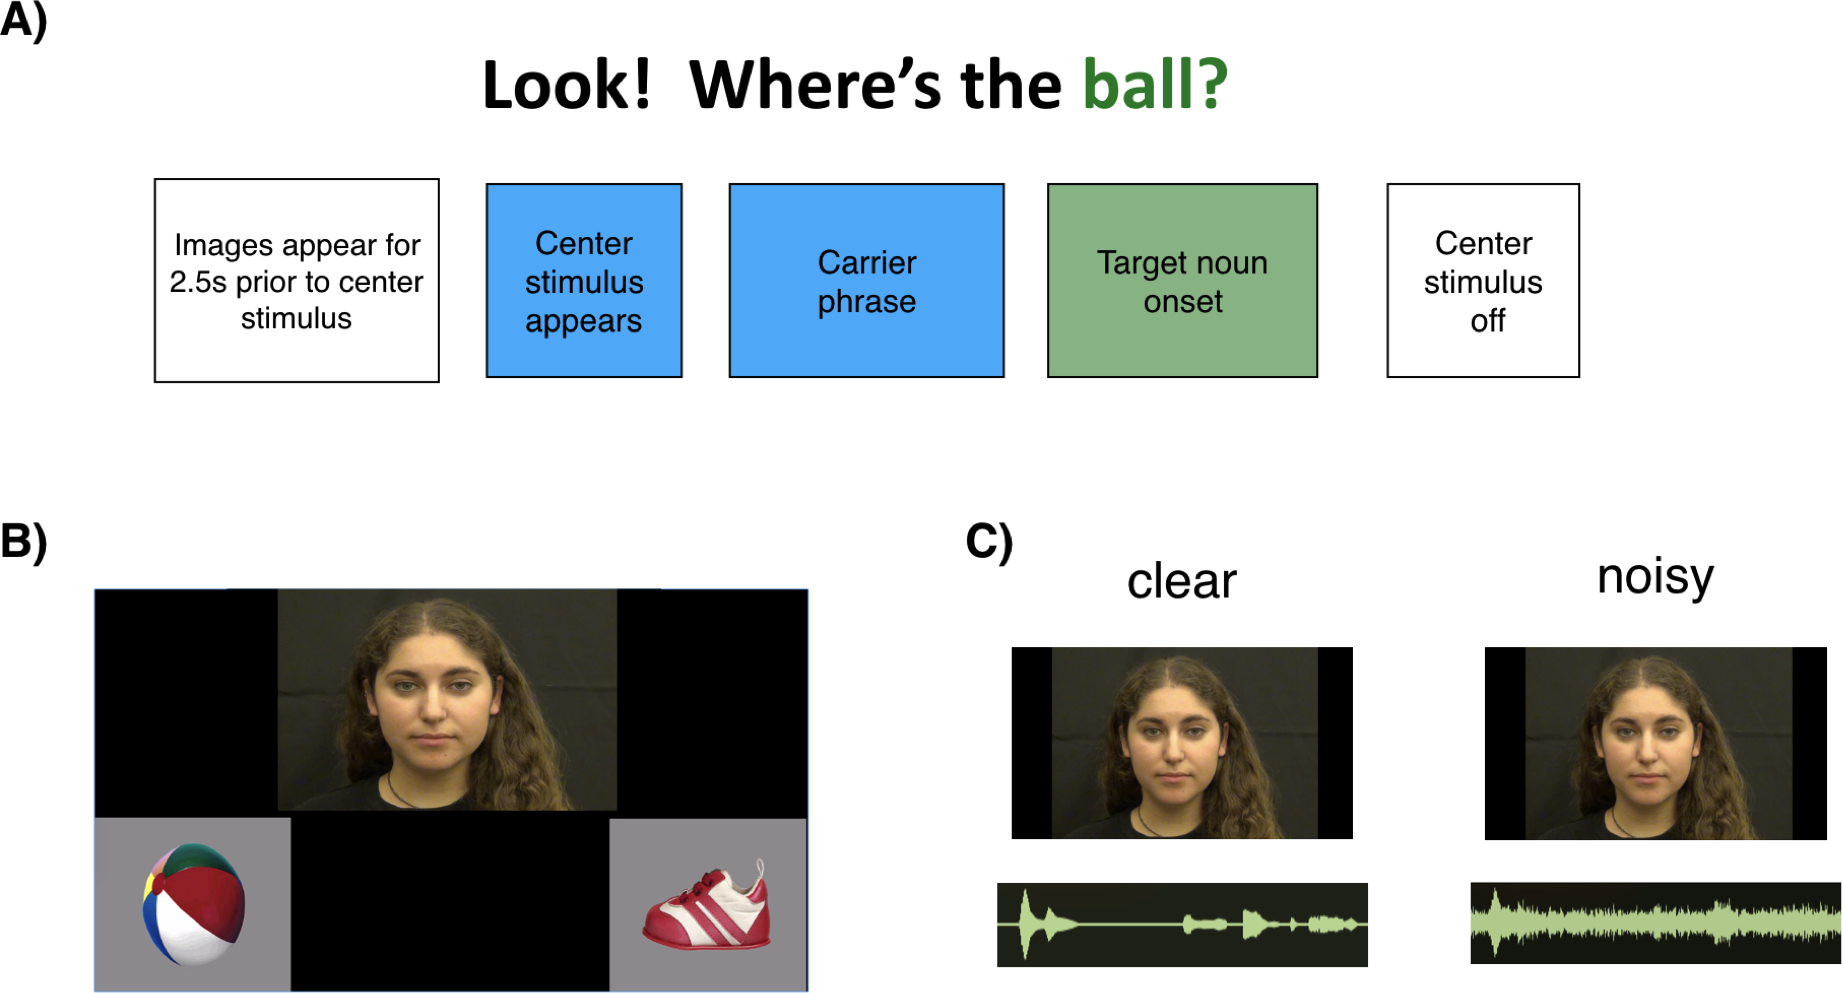
\includegraphics[width=0.8\linewidth]{figs/stimuli-plot-1} 

}

\caption{Experimental design and stimuli. Panel A shows the timecourse of the linguistic stimuli for a single trial. Panel B shows the layout of the three fixation locations (speaker, target, and distracter). Panel C shows a visual representation of the clear and noisy waveforms.}\label{fig:stimuli-plot}
\end{figure}

Here, we synthesize these ideas and test the generality of our
information-seeking account of eye movements during grounded language
comprehension. We ask whether listeners will adapt the timing of gaze
shifts away from a speaker if the auditory signal is less reliable -- as
is the case when processing speech in a noisy environment.

The second goal of this work is to test whether children show a similar
pattern of behavior and flexibly adapt fixations in response to changes
in the utility of gathering certain kinds of visual information. Recent
developmental work shows that, like adults, preschoolers will flexibly
adjust how they interpret ambiguous sentences (e.g., \enquote{I had
carrots and \emph{bees} for dinner.}) by integrating information about
the reliability of the incoming perceptual information with their
expectations about the speaker (Yurovsky, Case, \& Frank, 2017). While
children's behavior paralleled adults, they relied more on top-down
expectations about the speaker, perhaps because their developing
perceptual representations were noisier compared with adults. These
developmental differences provide insight into how children succeed in
understanding language despite having partial knowledge of word-object
links and without a fully-developed language model.

In our experiment, we hypothesized that a noisy auditory environment
increases the value of fixating a speaker to gather visual information
that supports comprehension. Our key behavioral prediction is that
listeners in noisy contexts will delay generating an eye movement away
from a speaker until they have accumulated additional visual information
about the identity of the named referent. This delay, in turn, will lead
to fewer random gaze shifts to the rest of the visual world. We also
predicted that preschoolers would show a parallel pattern of adaptation
to noisy contexts and allocate more fixations to a speaker's face when
it became more useful for accurate language comprehension. A plausible
alternative to our hypothesis is that the effects of language on visual
attention are so well-practiced that we would not see listeners adapt
their gaze patterns to the processing context.

To quantify the evidence for our predictions, we analyze the accuracy
and reaction times (RTs) of listeners' first gaze shifts after hearing
the name of an object in the visual scene. We focus on first shifts
because they provide a window onto changes in the underlying dynamics of
decision processes that generate eye movements.

\section{Experiment 1}\label{experiment-1}

Experiment 1 provides an initial test of our adaptive tradeoffs account.
We compared eye movements of children learning ASL to children learning
a spoken language using parallel real-time language comprehension tasks
where children processed familiar sentences (e.g., \enquote{Where's the
ball?}) while looking at a simplified visual world with 3 fixation
targets (a center stimulus that varied by condition, a target picture,
and a distracter picture; see Fig 1). The spoken language data are a
reanalysis of three unpublished data sets, and the ASL data are reported
in MacDonald et al. (under review). We predicted that, compared to
spoken language processing, processing ASL would increase the value of
fixating on the language source and decrease the value of generating
exploratory, nonlanguage-driven shifts even after the target linguistic
item began unfolding in time.

To test this prediction, we present traditional behavioral analyses of
first shift Accuracy and RT. We also present two model-based analyses.
First, we use an exponentially weighted moving average (EWMA) method
(Vandekerckhove \& Tuerlinckx, 2007) to categorize participants' gaze
shifts as language-driven or random. In contrast to the standard
RT/Accuracy analysis, the EMWA allows us to quantify differences in the
accuracy of gaze shifts as a function of \emph{when} that shift occurred
in time. Next, we use drift-diffusion models (DDMs) (Ratcliff \&
Childers, 2015) to quantify differences in the underlying psychological
variables that might drive behavioral differences in Accuracy and RT.
For example, the DDM uses the shape of \emph{both} the correct and
incorrect RT distributions to provide a quantiative estimate of whether
higher accuracy is driven by more cautious responding or by more
efficient information processing.

\subsection{Analysis plan}\label{analysis-plan}

First, we present behavioral analyses of First Shift Accuracy and
Reaction Time (RT).\footnote{See \url{https://osf.io/g8h9r/} for a
  pre-registration of the analysis plan.} RT corresponds to the latency
to shift away from the central stimulus to either picture measured from
the onset of the target noun. Accuracy corresponds to whether
participants' first gaze shift landed on the target or the distracter
picture. However, it is important to point out that when we analyze
differences in accuracy, we are not making claims about the overall
amount of time spent looking at the target vs.~the distractor image -- a
measure typically used in analyses of the Visual World Paradigm.

We used the \texttt{rstanarm} (Gabry \& Goodrich, 2016) package to fit
Bayesian mixed-effects regression models. The mixed-effects approach
allowed us to model the nested structure of our data -- multiple trials
for each participant and item, and a within-participants manipulation --
by including random intercepts for each participant and item, and a
random slope for each item and noise condition. We used Bayesian
estimation to quantify uncertainty in our point estimates, which we
communicate using a 95\% Highest Density Interval (HDI). The HDI
provides a range of credible values given the data and model. Finally,
to estimate age-related differences, we fit two types of models: (1) age
group (adults vs.~children) as a categorical predictor and (2) age (in
days) as a continuous predictor within the child sample.

Next, we present the two model-based analyses -- the EWMA and DDM. The
goal of these models is to move beyond a description of the data and map
behavioral differences in eye movements to underlying psychological
variables. The EWMA method models changes in random shifting behavior as
a function of RT. For each RT, the model generates two values: a
\enquote{control statistic} (CS, which captures the running average
accuracy of first shifts) and an \enquote{upper control limit} (UCL,
which captures the pre-defined limit of when accuracy would be
categorized as above chance level). Here, the CS is an expectation of
random shifting to either the target or the distracter image
(nonlanguage-driven shifts), or a Bernoulli process with probability of
success 0.5. As RTs get slower, we assume that participants have
gathered more information and should become more accurate
(language-driven), or a Bernoulli process with probability success
\textgreater{} 0.5. Using this model, we can quantify the proportion of
gaze shifts that were language-driven as opposed to random responding.

Following Vandekerckhove and Tuerlinckx (2007), we selected shifts
categorized as language-driven by the EWMA and fit a hierarchical
Bayesian drift-diffusion model (HDDM). The DDM quantifies differences in
the underlying decision process that lead to different patterns of
behavior. The model assumes that people accumulate noisy evidence in
favor of one alternative with a response generated when the evidence
crosses a pre-defined decision threshold. Here, we focus on two
parameters of interest: \emph{boundary separation}, which indexes the
amount of evidence gathered before generating a response (higher values
suggest more cautious responding) and \emph{drift rate}, which indexes
the amount of evidence accumulated per unit time (higher values suggest
more efficient processing).

Note:\footnote{We, furthermore, used the R-packages \emph{here} (0.1,
  Müller, 2017), \emph{knitr} (1.18, Xie, 2015), \emph{papaja}
  (0.1.0.9492, Aust \& Barth, 2017), \emph{rstanarm} (2.17.2, Stan
  Development Team, 2016), and \emph{tidyverse} (1.2.1, Wickham, 2017).}

\subsection{Methods}\label{methods}

\subsubsection{Participants}\label{participants}

\begin{table}[b]
\centering
\begin{tabular}{lrrrr}
  \hline
Task & Mean\_Age & Min\_Age & Max\_Age & n \\ 
  \hline
ASL & 27.90 & 16.00 & 53.00 &  30 \\ 
  Face & 26.00 & 25.00 & 26.00 &  24 \\ 
  Object & 31.90 & 26.00 & 39.00 &  40 \\ 
  Bullseye & 26.10 & 26.00 & 27.00 &  16 \\ 
   \hline
\end{tabular}
\caption{Age distributions of children in Experiment 1. All ages are reported in months.} 
\end{table}

Table 1 contains details about the age distributions of children in all
of four samples.

\emph{Spoken English samples.} Participants were 80 native, monolingual
English-learning children divided across three samples. Participants had
no reported history of developmental or language delay.

\emph{ASL sample.} Participants were 30 native, monolingual ASL-learning
children (18 deaf, 12 hearing). All children, regardless of hearing
status, were exposed to ASL from birth through extensive interaction
with at least one caregiver fluent in ASL and were reported to
experience at least 80\% ASL in their daily lives. The ASL sample
included a wider age range compared to the spoken English samples
because this is a rare population.

\subsubsection{Stimuli}\label{stimuli}

\emph{ASL linguistic stimuli.} We recorded two sets of ASL stimuli,
using two valid ASL sentence structures for questions: 1)
Sentence-initial wh-phrase: \enquote{HEY! WHERE {[}target noun{]}?} and
2) Sentence-final wh-phrase: \enquote{HEY! {[}target noun{]} WHERE?} Two
female native ASL users recorded several tokens of each sentence in a
child-directed register. Before each sentence, the signer produced a
common attention-getting gesture. Mean sign length was 1.25 sec, ranging
from 0.69 sec to 1.98 sec.

\emph{English linguistic stimuli.} All three tasks (Object, Bullseye,
and Face) featured the same female speaker who used natural
child-directed speech and said: \enquote{Look! Where's the (target
word)?} The target words were: ball, banana, book, cookie, juice, and
shoe. For the Face task, a female native English speaker was
video-recorded as she looked straight ahead and said, \enquote{Look!
Where's the (target word)?} Mean word length was 0.79 sec, ranging from
0.60 sec to 0.94 sec.

\emph{ASL and English visual stimuli.} The image set consisted of
colorful digitized pictures of objects presented in fixed pairs with no
phonological overlap (ASL task: cat---bird, car---book, bear---doll,
ball---shoe; English tasks: book-shoe, juice-banana, cookie-ball). Side
of target picture was counterbalanced across trials.

\subsubsection{Design and procedure}\label{design-and-procedure}

Children sat on their caregiver's lap and viewed the task on a screen
while their gaze was recorded using a digital camcorder. On each trial,
children saw two images of familiar objects on the screen for two
seconds before the center stimulus appeared (see Fig 1). Then they
processed the target sentence -- which consisted of a carrier phrase, a
target noun, and a question -- followed by two seconds without language
to allow for a response. Participants saw 32 test trials with several
filler trials interspersed to maintain interest.

\emph{Coding.} Participants' gaze patterns were coded (33-ms resolution)
as being fixated on either the center stimulus, one of the images,
shifting between pictures, or away. To assess inter-coder reliability,
25\% of the videos were re-coded. Agreement was scored at the level of
individual frames of video and averaged 98\% on these reliability
assessments.

\subsection{Results and discussion}\label{results-and-discussion}

\subsection{Results and Discussion}\label{results-and-discussion-1}

\begin{figure}[tb]

{\centering 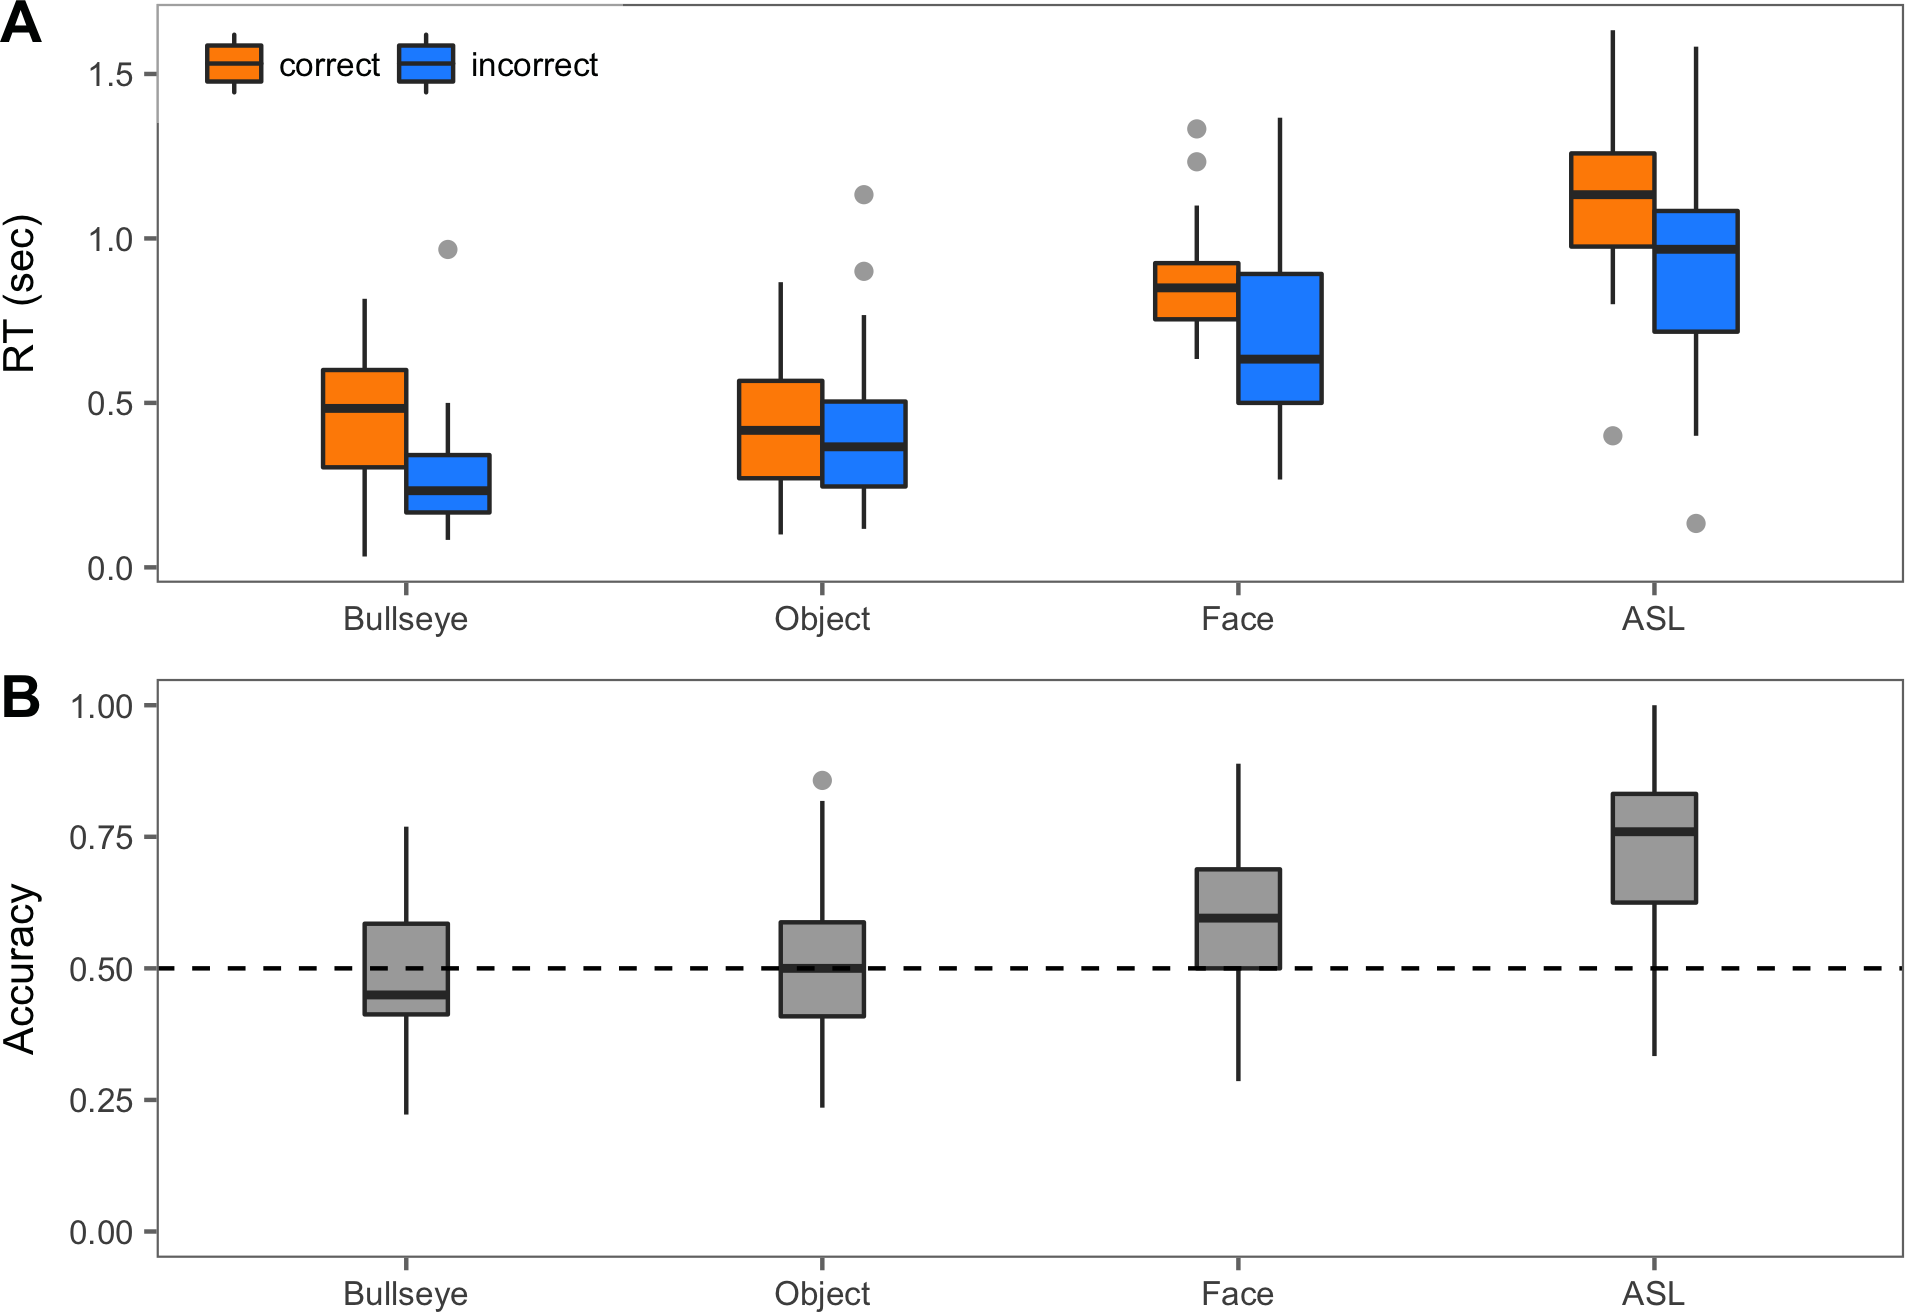
\includegraphics[width=0.8\linewidth]{figs/trio-plot-behav-1} 

}

\caption{First shift accuracy and RTs from Experiment 1. Panel A shows a boxplot representing the distribution of RTs for correct (orange) and incorrect (blue) shifts for each center stimulus type. Panel B shows the distribution of mean first shift accuracy scores for each center stimulus type. The solid lines represent median values, the boundaries of the box show the upper and lower quartiles, and the whiskers show the full range of the data excluding outliers.}\label{fig:trio-plot-behav}
\end{figure}

\subsubsection{Behavioral analyses}\label{behavioral-analyses}

\emph{RT.} Visual inspection of the Fig 2, panel A suggests that there
was a speed accuracy tradeoff in the ASL, Face, and Bullseye conditions,
with incorrect shifts tending to be faster than correct shifts. To
quantify differences across the groups, we fit a linear mixed-effects
regression predicting first shift RT as a function of center stimulus
type, controlling for age, and including user-defined contrasts to test
specific comparisons of interest:
\texttt{Log(RT) $\sim$ center stimulus type + age +  (1 | subject) + (1 | item)}.
We found that (a) ASL learners generated slower RTs compared to all of
the spoken English samples (\(\beta\) = -0.97, \(p\) \textless{} .001),
(b) ASL learners' shifts were slower compared directly to participants
in the Face task (\(\beta\) = -0.42, \(p\) \textless{} .001), and (c)
participants in the Face task shifted slower compared to participants in
the Object and Bullseye tasks (\(\beta\) = -0.73, \(p\) \textless{}
.001).

\emph{Accuracy.} Next we compared the accuracy of first shifts across
the different tasks by fitting a mixed-effects logistic regression with
the same specifications and contrasts as the RT model. We found that (a)
ASL learners were more accurate compared to all of the spoken English
samples (\(\beta\) = -0.78, \(p\) \textless{} .001), (b) ASL learners
were more accurate when directly compared to participants in the Face
task (\(\beta\) = -0.62, \(p\) = 0.001), and (c) participants in the
Face task were numerically more accurate compared to participants in the
Object and Bullseye tasks (\(\beta\) = -0.73) but this effect was not
significant (\(p\) = 0.089).

\subsubsection{Model-based analyses}\label{model-based-analyses}

\begin{figure}[tb]

{\centering 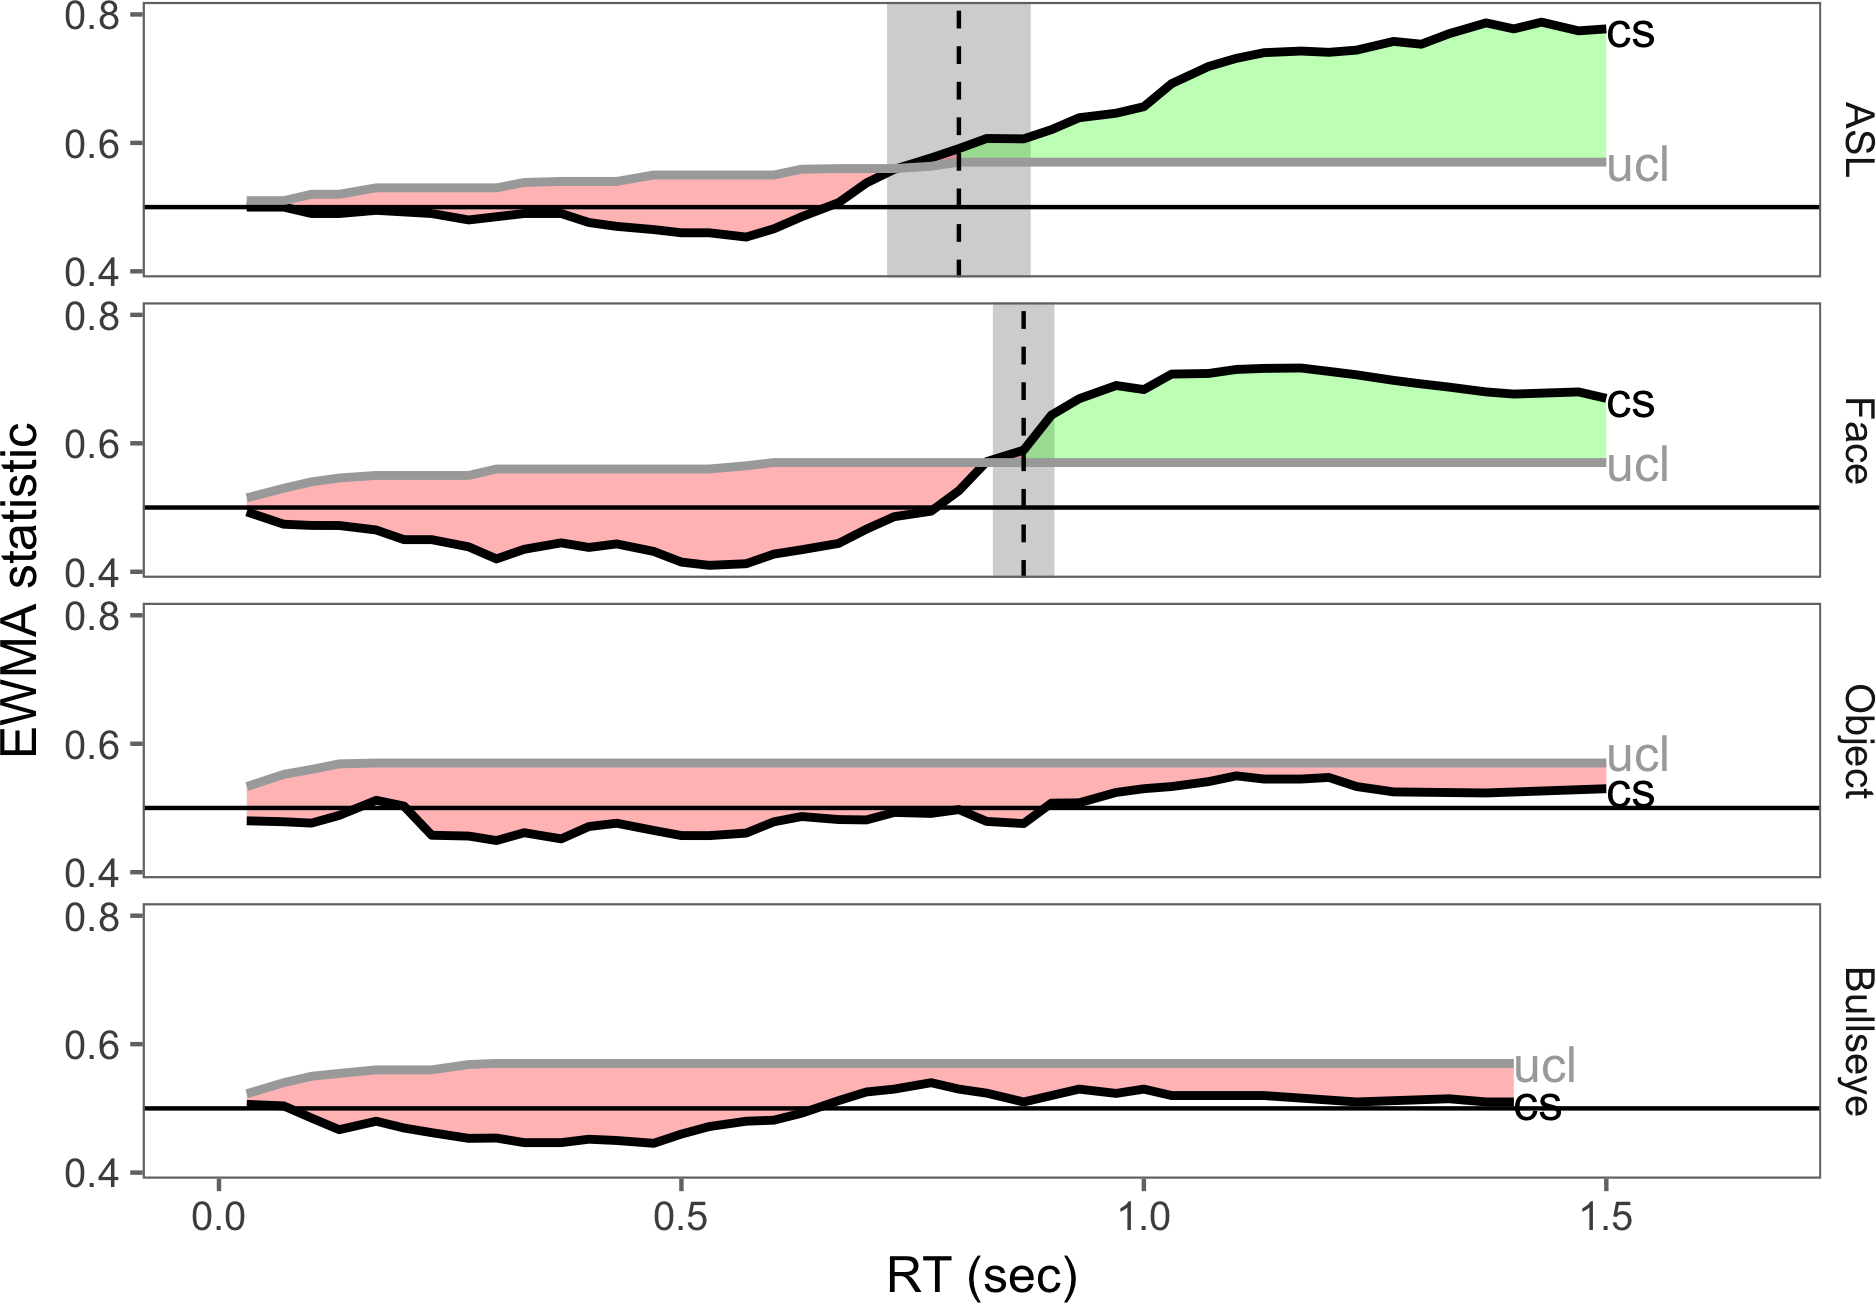
\includegraphics[width=0.8\linewidth]{figs/trio-control-plot-1} 

}

\caption{Output for the EWMA guessing model in E1. The black curve represents the evolution of the control statistic (CS) as a function of reaction time. The grey curve represents the upper control limit (UCL). The vertical dashed line is the median cutoff value (point when the control process shifts out of a guessing state). The grey shaded area represents the 95\% confidence interval around the estimate of the median cutoff point. And the shaded areas represents the proprotion of responses that were flagged as guesses (red) and language-driven (green).}\label{fig:trio-control-plot}
\end{figure}

\emph{EWMA.} Figure 3 shows changes in the control statistic (CS) and
the upper control limit (UCL) as a function of participants' RTs. Each
CS starts at chance performance and below the UCL. In the ASL and Face
tasks, the CS value begins to increase with RTs around 0.7 seconds after
noun onset and eventually crosses the UCL, indicating that responses
\textgreater{} 0.7 sec were on average above chance levels. In contrast,
the CS in the Object and Bullseye tasks never crossed the UCL,
indicating that children's shifts were equally likely to land on the
target or the distracter, regardless of when they were initiated. This
result suggests that first shifts in the Bullseye/Object tasks were not
language-driven and may instead have reflected a different process such
as gathering more information about the referents in the visual world.

Next, we compared the EWMA output for participants in the ASL and Face
tasks. We found that ASL learners generated fewer shifts when the CS was
below the UCL (\(\beta\) = -1.65, \(p\) \textless{} .001), indicating
that a larger proportion of their initial shifts away were
language-driven (see the differences in the red shaded area in Fig 3).
We did not find evidence for a difference in the timing of when the CS
crossed the UCL (\(\beta\) = -0.04, \(p\) = 0.331), indicating that both
groups began to generate language-driven shifts about the same time
after noun onset.

\begin{figure}[tb]

{\centering 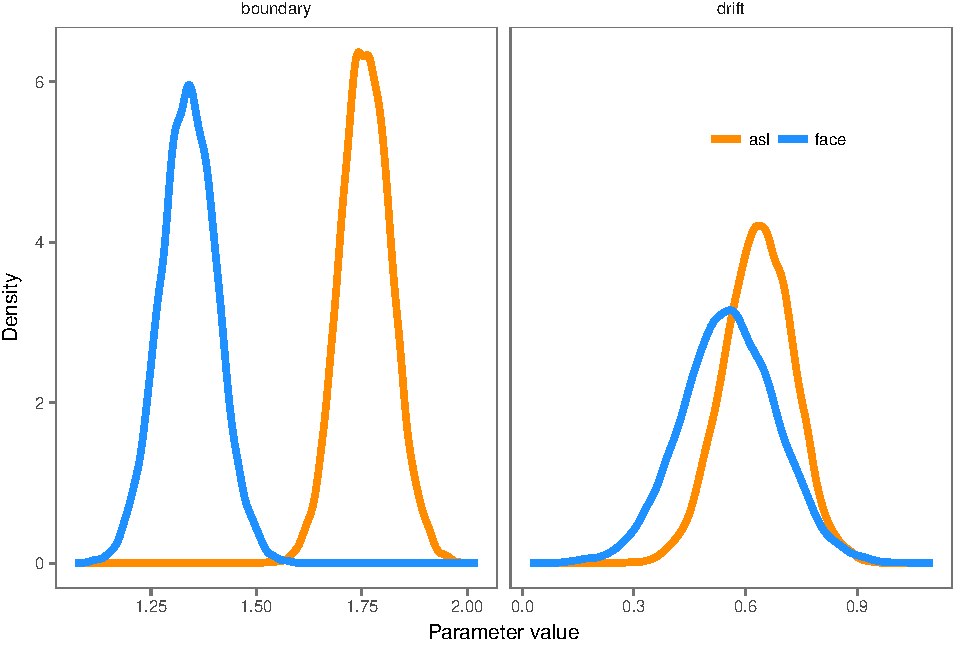
\includegraphics[width=0.8\linewidth]{figs/trio-hddm-plot-1} 

}

\caption{Posterior distributions for the boundary and drift rate parameters for children in Experiment 1.}\label{fig:trio-hddm-plot}
\end{figure}

\emph{HDDM.} Using the output of the EWMA, we compared the timing and
accuracy of language-driven shifts for participants in the ASL and Face
tasks.\footnote{We report the mean and the 95\% highest density interval
  (HDI) of the posterior distributions for each parameter. The HDI
  represents the range of credible values given the model specification
  and the data. We chose not to interpret the DDM fits for the
  Bullseye/Face tasks since there was no suggestion of any non-guessing
  signal.} We found that ASL learners had a higher estimate for the
boundary separation parameter compared to the Face participants (ASL
boundary = 1.76, HDI = {[}1.64, 1.88{]}; Face boundary = 1.34, HDI =
{[}1.21, 1.47{]}), with no overlap in the credible values (see Fig 4).
This suggests that ASL learners accumulated more evidence about the
linguistic signal before generating an eye movement. We found high
overlap for estimates of the drift rate parameter, indicating that both
groups processed the linguistic information with similar efficiency (ASL
drift = 0.63, HDI = {[}0.45, 0.82{]}; Face drift = 0.56, HDI = {[}0.30,
0.81{]}).

Taken together, the behavioral analyses and the EWMA/HDDM results
provide converging support that ASL learners were sensitive to the value
of eye movements, producing fewer nonlanguage-driven shifts and
prioritizing accuracy over speed, but accumulating information at
roughly the same rate. This behavior seems reasonable since the
potential for missing subsequent linguistic information is high if ASL
users shifted prior to gathering sufficient information. It is important
to point out that these were exploratory findings and that there were
several, potentially important differences between the stimuli,
apparatus, and populations. In Experiment 2, we set out to perform a
well-controlled, confirmatory test of our adaptive tradeoffs account.

\section{Experiment 2}\label{experiment-2}

In Experiment 2, we attempt to replicate a key finding from Experiment
1: that increasing the competition between fixating the language source
and the nonlinguistic visual world reduces nonlanguage-driven eye
movements. Moreover, we conducted a confirmatory test of our hypothesis
that also controlled for the population differences present in
Experiment 1. We tested a sample of English-speaking adults using a
within-participants manipulation of the center stimulus type. We used
the Face and Bullseye stimulus sets from Experiment 1 and added two new
conditions: Text, where the verbal language information was accompanied
by a word-by-word display of printed text (see Fig 1), and
Text-no-audio, where the spoken language stimulus was removed. We chose
text processing since, like sign language comprehension, the linguistic
information is gathered via fixations to the visual world.

Our key behavioral prediction is that participants in the Text
conditions should produce a higher proportion of language-driven shifts
as indexed by the EWMA model output. We did not have strong predictions
for the DDM parameter fits since the goal of the Text manipulation was
to modulate participants' strategic allocation of visual attention and
not the accuracy/efficiency of information processing.

\subsection{Methods}\label{methods-1}

\subsubsection{Participants}\label{participants-1}

25 Stanford undergraduates participated (5 male) for course credit. All
participants were monolingual, native English speakers and had normal
vision.

\subsubsection{Stimuli}\label{stimuli-1}

Audio and visual stimuli were identical to the Face and Bullseye tasks
in Experiment 1. We included a new center fixation stimulus type:
printed text. The text was displayed in a white font on a black
background and was programmed such that only a single word appeared on
the screen, with each word appearing for the same duration as the
corresponding word in the spoken language stimuli.

\subsubsection{Design and procedure}\label{design-and-procedure-1}

The design was nearly identical to Experiment 1, with the exception of a
change to a within-subjects manipulation where each participant
completed all four tasks (Bullseye, Face, Text, and Text-no-audio). In
the Text condition, spoken language accompanied the printed text. In the
Text-no-audio condition, the spoken language stimulus was removed.
Participants saw a total of 128 trials while their eye movements were
tracked using automated eye-tracking software.

\subsection{Results and Discussion}\label{results-and-discussion-2}

\begin{figure}[t]

{\centering 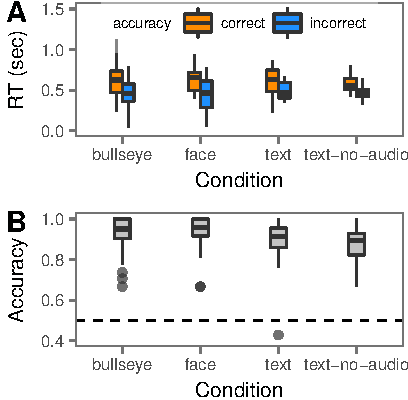
\includegraphics[width=0.8\linewidth]{figs/text-plot-print-1} 

}

\caption{Behavioral results for Experiment 2. All plotting conventions are the same as in Figure 2.}\label{fig:text-plot-print}
\end{figure}

\subsubsection{Behavioral analyses}\label{behavioral-analyses-1}

\emph{RT.} Visual inspection of Figure 5, panel A suggests that there
was a speed-accuracy tradeoff for all conditions: incorrect gaze shifts
tended to be faster than correct shifts. We fit a linear mixed-effects
regression with the same specification as in Experiment 1, but we added
by-subject intercepts and slopes for each center stimulus type to
account for our within-subjects manipulation. We did not find evidence
that RTs were different across conditions (all \(p\) \textgreater{}
.05).

\emph{Accuracy.} Next, we modeled accuracy using a mixed-effects
logistic regression with the same specifications (see Panel B of Fig 5).
We found that adults' first shifts were highly accurate, and, in
contrast to the children in Experiment 1, their responses were above
chance level even in the Bullseye condition when the center stimulus was
not salient or informative. We also found that participants tended to be
less accurate in the Text conditions compared to conditions without text
(\(\beta\) = 1.18, \(p\) = 0.00). We did find not any other
statistically significant differences.

\subsubsection{Model-based analyses}\label{model-based-analyses-1}

\begin{figure}[tb]

{\centering 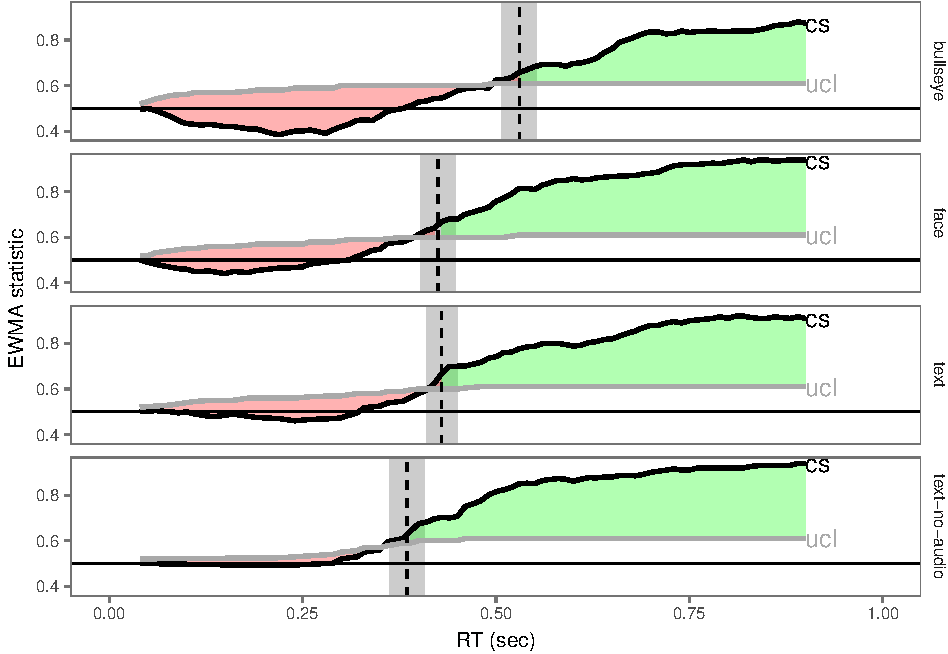
\includegraphics[width=0.8\linewidth]{figs/text-ewma-plot-1} 

}

\caption{EWMA model output for Experiment 2. All plotting conventions are the same as Figure 3.}\label{fig:text-ewma-plot}
\end{figure}

\emph{EWMA.} For all four conditions, the CS crossed the UCL (see Fig
6), suggesting that for all tasks some proportion of adults' shifts were
language-driven. Interestingly, we found a graded effect of condition
(see the shift in the vertical dashed lines in Fig 5) on the point when
the CS crossed the UCL such that the Text-no-audio condition occurred
earliest (\(M_{text-no-audio}\) = 0.39), followed by the Text and Face
conditions that were not different from one another (\(M_{text}\) =
0.44, \(M_{face}\) = 0.45, \(p\) \textgreater{} .05), and finally the
Bullseye condition (\(M_{bullseye}\) = 0.54). We also found the same
graded difference in the proportion of shifts that occurred while the CS
was below the UCL (see the red vs.~green shaded area in Fig 5),
indicating a higher proportion of first shifts were language-driven in
the Text conditions, with the highest proportion in the Text-no-audio
condition when tested against the three other conditions
(\(M_{text-no-audio}\) = 3.79, \(\beta\) = 1.74, \(p\) \textless{}
.001). These results provide strong evidence for our key prediction:
that increasing the value of fixating the language source reduces
exploratory gaze shifts to the nonlinguistic visual world.

\begin{figure}[tb]

{\centering 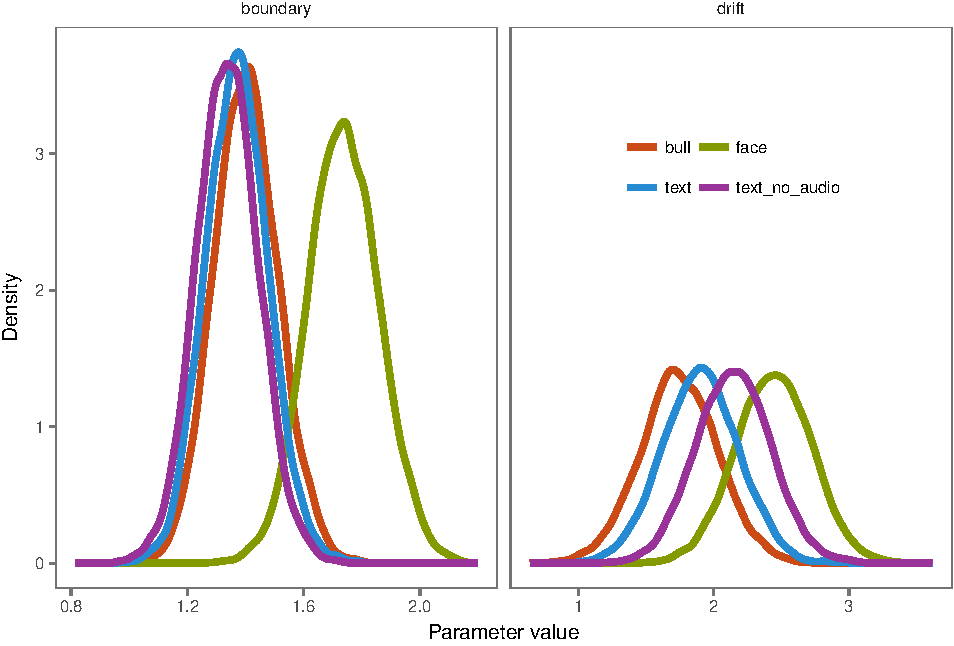
\includegraphics[width=0.8\linewidth]{figs/text-hddm-plot-1} 

}

\caption{Posterior distributions for the boundary and drift rate parameters for Experiment 2.}\label{fig:text-hddm-plot}
\end{figure}

\emph{HDDM.} Using the output of the EWMA, we fit the same HDDM as in
Experiment 1. There was high overlap of the posterior distributions for
the drift rate parameters (see Fig 4, panel B), suggesting that
participants gathered the linguistic information with similar
efficiency. We also found high overlap in the distribution of credible
boundary separation estimates for the Bullseye, Text, and Text-no-audio
conditions. Interestingly, we found some evidence for a higher boundary
separation in the Face condition compared to the other three center
stimulus types (Face boundary = 1.74, HDI = {[}1.50, 1.98{]}; Bullseye
boundary = 1.40, HDI = {[}1.19, 1.63{]}; Text boundary = 1.37, HDI =
{[}1.16, 1.59{]}; Text-no-audio boundary = 1.34, HDI = {[}1.13,
1.55{]}), suggesting that adults higher accuracy in this condition was
driven by accumulating more information before generating a response.

Together, these results suggest that adults were sensitive to the
tradeoff between gathering different kinds of information. When
processing text, people generated fewer nonlanguage-driven shifts (EWMA
results) but their processing efficiency of the linguistic signal itself
did not change (HDDM results). Interestingly, we found a graded
difference in the EWMA results between the Text and Text-no-audio
conditions, with the lowest proportion of early, nonlanguage-driven
shifts occurring while processing text without the verbal stimuli. This
behavior makes sense; if the adults could rely on the auditory channel
to gather the linguistic information, then the value of fixating the
text display decreases. In contrast to the children in Experiment 1,
adults were highly accurate in the Bullseye condition, perhaps because
they construed the Bullseye as a center fixation that they \emph{should}
fixate, or perhaps they had better encoded the location/identity of the
two referents prior to the start of the target sentence.

\section{Experiment 3}\label{experiment-3}

In this experiment, we recorded adults and children's eye movements
during a real-time language comprehension task where participants
processed familiar sentences (e.g., \enquote{Where's the ball?}) while
looking at a simplified visual world with three fixation targets (see
Fig.~\ref{fig:stimuli_plot}). Using a within-participants design, we
manipulated the signal-to-noise ratio of the auditory signal by
convolving the acoustic input with brown noise (random noise with
greater energy at lower frequencies).

First, we present standard behavioral analyses of reaction time (RT) and
accuracy of listeners' first gaze shifts after target noun onset. Then,
we present two model-based analyses that link observable behavior to
underlying psychological constructs. We use an exponentially weighted
moving average (EWMA) method (Vandekerckhove \& Tuerlinckx, 2007) to
classify participants' gaze shifts as language-driven or random. In
contrast to the standard RT/accuracy analysis, the EMWA approach allows
us to quantify participants' willingness to generate gaze shifts after
noun onset but before collecting sufficient information to seek the
named referent. Higher values indicate that participants were waiting to
shift until they had accumulated enough of the linguistic signal to
locate the named referent. Finally, we use drift-diffusion models (DDMs)
(Ratcliff \& Childers, 2015) to ask whether behavioral differences in
accuracy and RT are driven by a more cautious responding strategy or by
more efficient information processing.

We predicted that processing speech in a noisy context would make
participants less likely to shift before collecting sufficient
information. This delay, in turn, would lead to a lower proportion of
shifts flagged as random/exploratory in the EWMA analysis, and a pattern
of DDM results indicating a prioritization of accuracy over and above
speed of responding (see the Analysis Plan section below for more
details on the models). We also predicted a developmental difference --
that children would produce a higher proportion of random shifts and
accumulate information less efficiently compared to adults; and a
developmental parallel -- that children would show the same pattern of
adapting gaze patterns to gather more visual information in the noisy
processing context.

\subsection{Methods}\label{methods-2}

\subsubsection{Participants}\label{participants-2}

Participants were native, monolingual English-learning children (\(n=\)
39; 22 F) and adults (\(n=\) 31; 22 F). All participants had no reported
history of developmental or language delay and normal vision. 14
participants (11 children, 3 adults) were run but not included in the
analysis because either the eye tracker falied to calibrate (2 children,
3 adults) or the participant did not complete the task (9 children).

\subsubsection{Stimuli}\label{stimuli-2}

\emph{Linguistic stimuli.} The video/audio stimuli were recorded in a
sound-proof room and featured two female speakers who used natural
child-directed speech and said one of two phrases: \enquote{Hey! Can you
find the (target word)} or ``Look! Where's the (target word) -- see
panel A of Fig.~\ref{fig:stimuli_plot}. The target words were: ball,
bunny, boat, bottle, cookie, juice, chicken, and shoe. The target words
varied in length (shortest = 411.68 ms, longest = 779.62 ms) with an
average length of 586.71 ms.

\emph{Noise manipulation}. To create the stimuli in the noise condition,
we convolved each recording with Brown noise using the Audacity audio
editor. The average signal-to-noise ratio\footnote{The ratio of signal
  power to the noise power, with values greater than 0 dB indicating
  more signal than noise.} in the noise condition was 2.87 dB compared
to the clear condition, which was 35.05 dB.

\emph{Visual stimuli.} The image set consisted of colorful digitized
pictures of objects presented in fixed pairs with no phonological
overlap between the target and the distractor image (cookie-bottle,
boat-juice, bunny-chicken, shoe-ball). The side of the target picture
was counterbalanced across trials.

\subsubsection{Design and procedure}\label{design-and-procedure-2}

Participants viewed the task on a screen while their gaze was tracked
using an SMI RED corneal-reflection eye-tracker mounted on an LCD
monitor, sampling at 60 Hz. The eye-tracker was first calibrated for
each participant using a 6-point calibration. On each trial,
participants saw two images of familiar objects on the screen for two
seconds before the center stimulus appeared (see
Fig.~\ref{fig:stimuli_plot}). Next, they processed the target sentence
-- which consisted of a carrier phrase, a target noun, and a question --
followed by two seconds without language to allow for a response. Child
participants saw 32 trials (16 noise trials; 16 clear trials) with
several filler trials interspersed to maintain interest. Adult
participants saw 64 trials (32 noise; 32 clear). The noise manipulation
was presented in a blocked design with the order of block
counterbalanced across participants.

\subsection{Results and discussion}\label{results-and-discussion-3}

\subsubsection{Behavioral analyses:}\label{behavioral-analyses-2}

\begin{figure}[tb]

{\centering 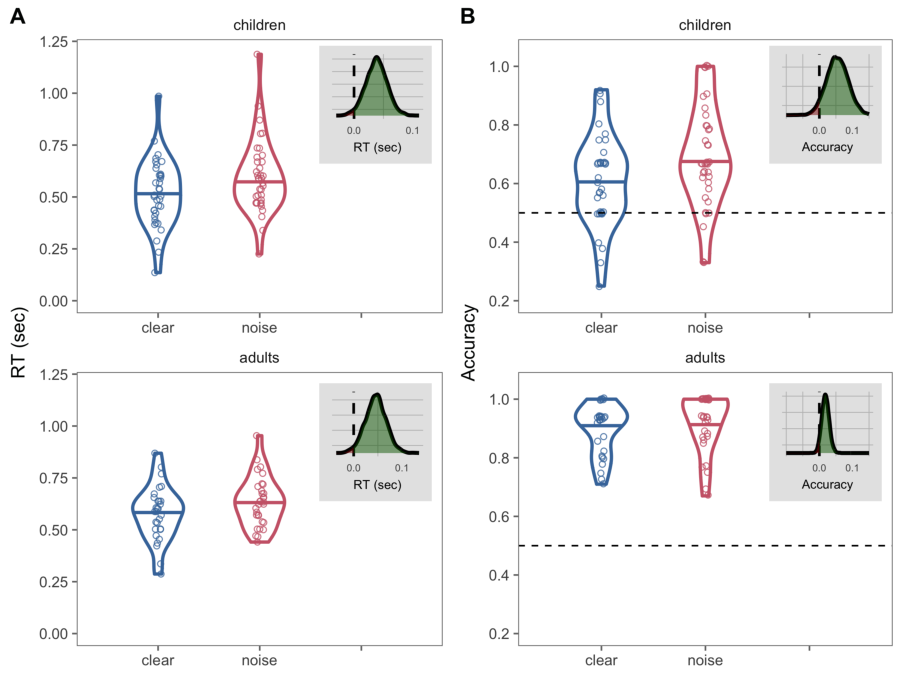
\includegraphics[width=0.8\linewidth]{figs/noise-acc-rt-1} 

}

\caption{Behavioral results for first shift Reaction Time (RT) and Accuracy. Panel A shows violin plots representing the distribution of RTs for each participant in each condition. Each point represents a participant's average RT. Color represents the processing context. The grey insets show the full posterior distribution of RT differences across conditions with the vertical dashed line representing the null value of zero condition difference. The green shading represents estimates in the predicted direction and above the null value while the red shading represents estimates below the null. Panel B shows the same information but for first shift accuracy.}\label{fig:noise-acc-rt}
\end{figure}

\textbf{RT.} To make RTs more suitable for modeling on a linear scale,
we analyzed responses in log space with the final model specified as:
\texttt{$log(RT) \sim noise\_condition + age\_group + (noise\_condition \mid sub\_id ) + (noise\_condition \mid target\_item)$}.
Panel A of Fig.~\ref{fig:noise_acc_rt_noise_plot} shows the full RT data
distribution and the full posterior distribution of the estimated RT
difference between the noise and clear conditions. Both children and
adults were slower to identify the target in the noise condition
(Children \(M_{noise}\) = 500.19 ms; Adult \(M_{noise}\) = 595.23 ms),
as compared to the clear condition (Children \(M_{clear}\) = 455.72 ms;
Adult \(M_{clear}\) = 542.45 ms). RTs in the noise condition were 48.82
ms slower on average, with a 95\% HDI ranging from 3.72 ms to 96.26 ms,
and not including the null value of zero condition difference. Older
children responded faster than younger children (\(M_{age}\) = -0.44,
{[}-0.74, -0.16{]}), with little evidence for an interaction between age
and condition.

\textbf{Accuracy.} Next, we modeled adults and children's first shift
accuracy using a mixed-effects logistic regression with the same
specifications (see Panel B of Fig.~\ref{fig:noise_acc_rt_noise_plot}).
Both groups were more accurate than a model of random responding (null
value of \(0.5\) falling well outside the lower bound of the 95\% HDI
for all group means). Adults were more accurate (\(M_{adults} =\) 90\%)
than children (\(M_{children} =\) 61\%). The key result is that both
groups showed evidence of higher accuracy in the noise condition:
children (\(M_{noise}\) = 67\%; \(M_{clear}\) = 61\%) and adults
(\(M_{noise}\) = 92\%; \(M_{clear}\) = 90\%). Accuracy in the noise
condition was on average 4\% higher, with a 95\% HDI from -1\% to 12\%.
Note that the null value of zero difference falls at the very edge of
the HDI. But 95\% of the credible values are greater than zero,
providing evidence for higher accuracy in the noise condition. Within
the child sample, there was no evidence of a main effect of age or an
interaction between age and noise condition.

\subsubsection{Model-based analyses:}\label{model-based-analyses-2}

\begin{figure}[tb]

{\centering 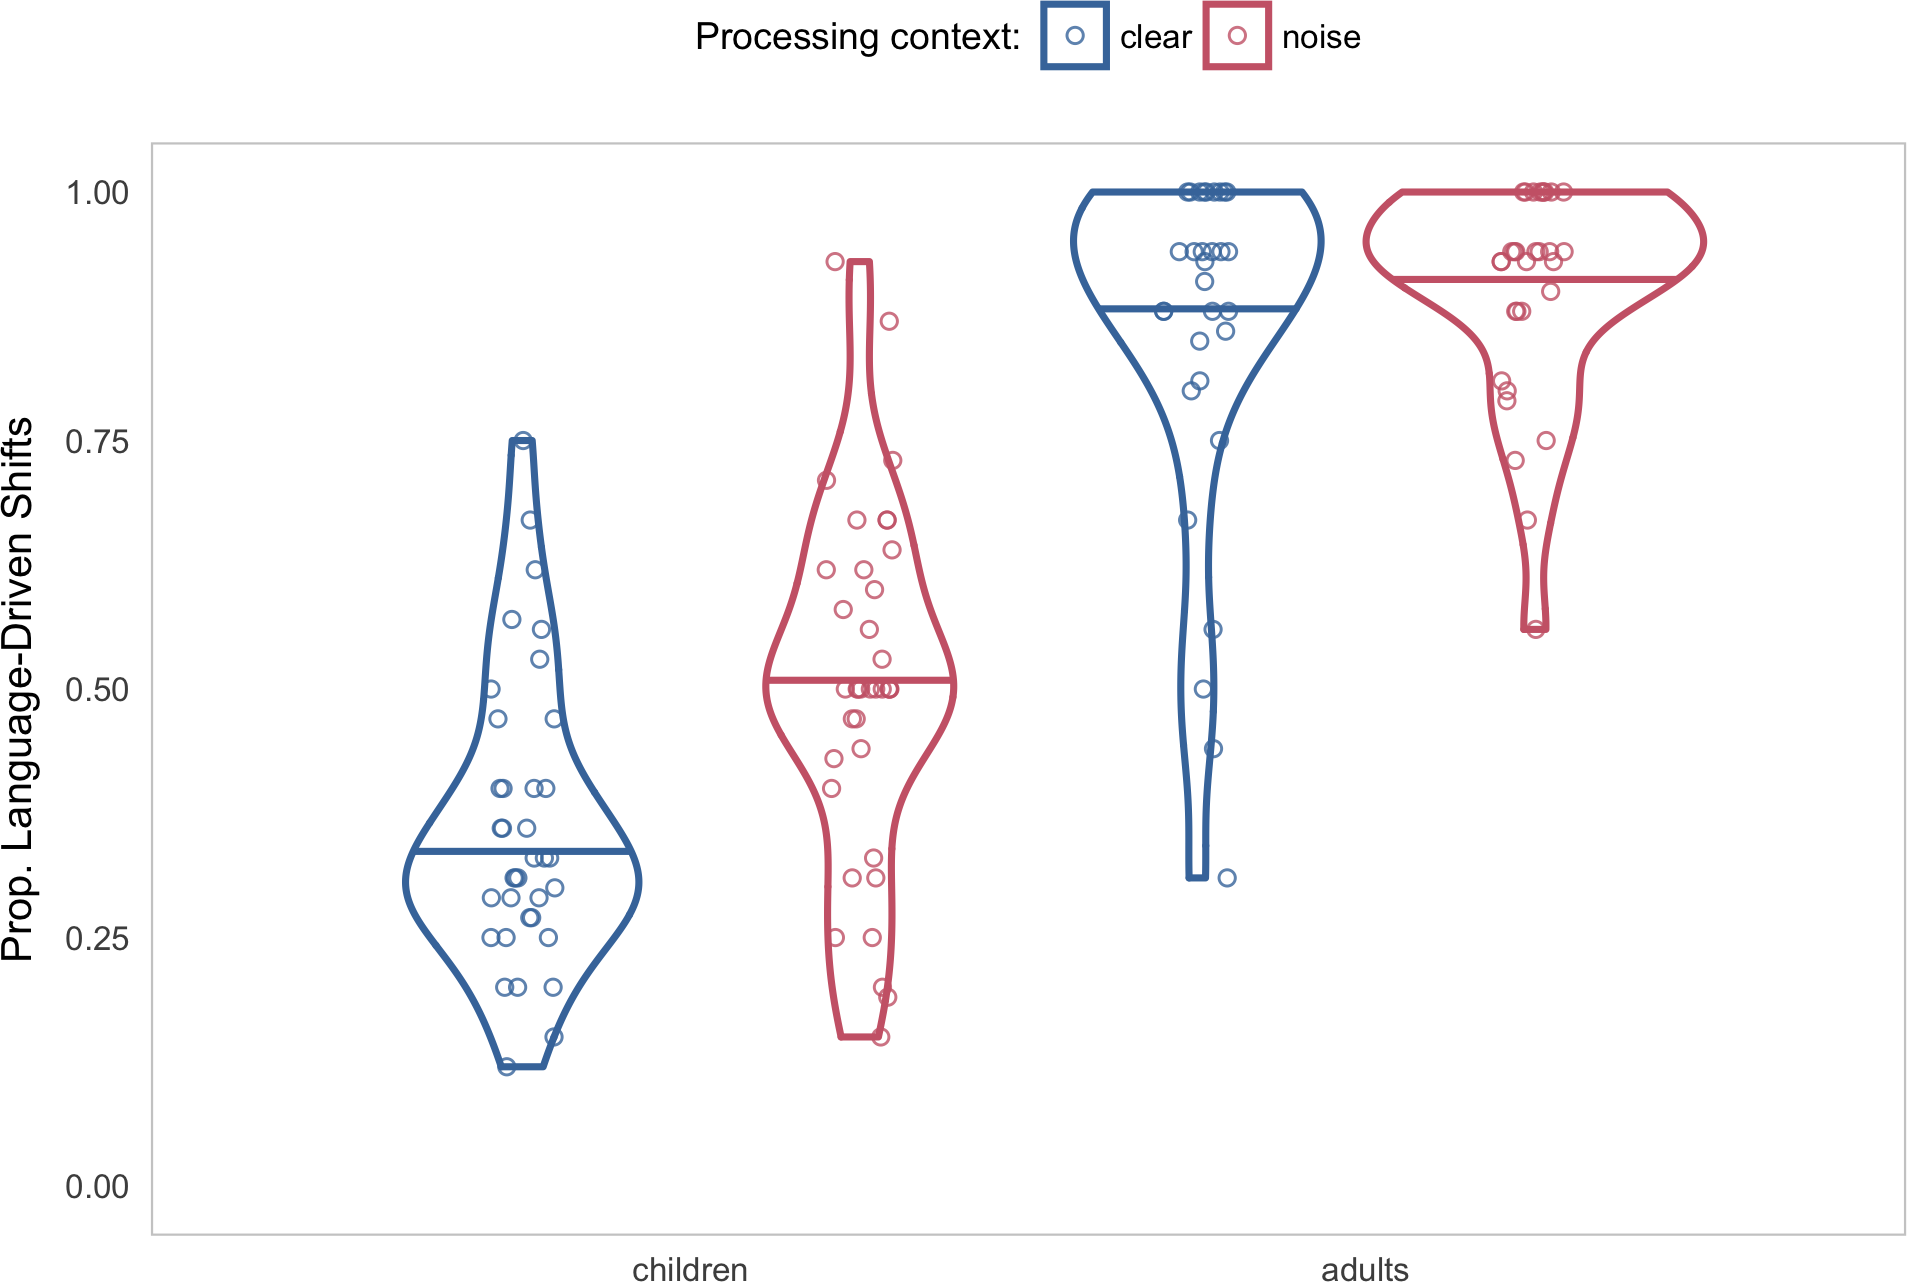
\includegraphics[width=0.8\linewidth]{figs/noise-violin-ewma-1} 

}

\caption{EWMA results for children and adults. Each point represents the proportion of shifts categorized as language-driven (as opposed to guessing) for a single participant. Color represents the processing context.}\label{fig:noise-violin-ewma}
\end{figure}

\textbf{EWMA.} Fig.~\ref{fig:noise_ewma_violin_plot} shows the
proportion of shifts that the model classified as random
vs.~language-driven for each age group and processing context. On
average, 41\% (95\% HDI: 32\%, 50\%) of children's shifts were
categorized as language-driven, which was significantly fewer than
adults, 87\% (95\% HDI: 78\%, 96\%). Critically, processing speech in a
noisy context caused both adults and children to generate a higher
proportion of language-driven shifts (i.e., fewer random, exploratory
shifts away from the speaker), with the 95\% HDI excluding the null
value of zero condition difference (\(\beta_{noise}\) = 11\%, {[}7.00\%,
16\%{]}). Within the child sample, older children generated fewer
random, early shifts (\(M_{age}\) = -0.21, {[}-0.35, -0.08{]}). There
was no eivdence of an interaction between age and condition. This
pattern of results suggests that the noise condition caused participants
to increase visual fixations to the language source, leading them to
generate fewer exploratory, random shifts before accumulating sufficient
information to respond accurately.

\begin{figure}[tb]

{\centering 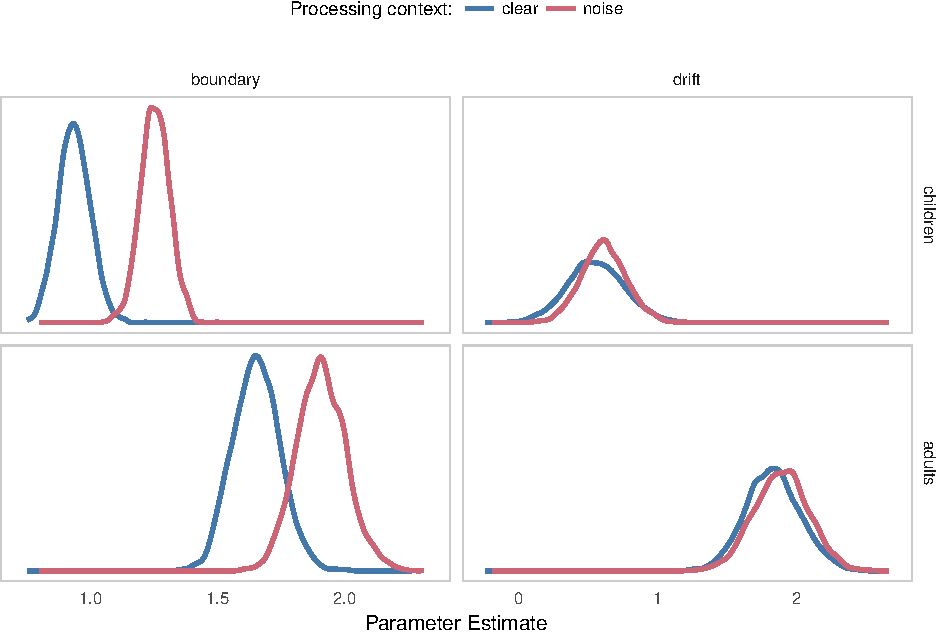
\includegraphics[width=0.8\linewidth]{figs/hddm-plot-noise-1} 

}

\caption{HDDM results. Each panel shows the posterior distribution for either the boundary separation or drift rate parameters for children (top panels) and adults (bottom panels).}\label{fig:hddm-plot-noise}
\end{figure}

\textbf{HDDM.} Fig.~\ref{fig:hddm_plot_noise} shows the full posterior
distributions for the HDDM output. Children had lower drift rates
(children \(M_{drift}\) = 0.58; adults \(M_{drift}\) = 1.90) and
boundary separation estimates (children \(M_{boundary}\) = 1.09; adults
\(M_{boundary}\) = 1.67) as compared to adults, suggesting that children
were less efficient and less cautious in their responding. The noise
manipulation selectively affected the boundary separation parameter,
with higher estimates in the noise condition for both age groups
(\(\beta_{noise}\) = 0.27, {[}0.11, 0.42{]}). This result suggests that
participants' in the noise condition prioritized information
accumulation over speed when generating an eye movement in response to
the incoming language. This increased decision threshold led to higher
accuracy. Moreover, the high overlap in estimates of drift rate suggests
that participants were able to integrate the visual and auditory signals
such that they could achieve a level of processing efficiency comparable
to the clear processing context.

Taken together, the behavioral and EWMA/HDDM results provide converging
support for the predictions of our information-seeking account.
Processing speech in noise caused listeners to seek additional visual
information to support language comprehension. Moreover, we observed a
very similar pattern of behavior in children and adults, with both
groups producing more language-driven shifts and prioritizing accuracy
over speed in the more challenging, noisy environment.

\section{General Discussion}\label{general-discussion}

Language comprehension in grounded contexts involves integrating
information from the visual and linguistic signals. But the value of
integrating visual information depends on the processing context. Here,
we presented a test of an information-seeking account of eye movements
during language processing: that listeners flexibly adapt gaze patterns
in response to the value of seeking visual information for accurate
language understanding. We showed that children and adults generate
slower but more accurate gaze shifts away from a speaker when processing
speech in a noisy context. Both groups showed evidence of prioritizing
information accumulation over speed (HDDM) while guessing less often
(EWMA). Listeners were able to achieve higher accuracy in the more
challenging, noisy context. Together, these results suggest that in
settings with a degraded linguistic signal, listeners support language
comprehension by seeking additional language-relevant information from
the visual world.

These results synthesize ideas from several research programs, including
work on language-mediated visual attention (Tanenhaus et al., 1995),
goal-based accounts of vision during everyday tasks (Hayhoe \& Ballard,
2005), and work on effortful listening (Van Engen \& Peelle, 2014).
Moreover, our findings parallel recent work by McMurray, Farris-Trimble,
and Rigler (2017) showing that individuals with Cochlear Implants, who
are consistently processing degraded auditory input, are more likely to
delay the process of lexical access as measured by slower gaze shifts to
named referents and fewer incorrect gaze shifts to phonological onset
competitors. McMurray et al. (2017) also found that they could replicate
these changes to gaze patterns in adults with typical hearing by
degrading the auditory stimuli so that it shared features with the
output of a cochlear implant (noise-vocoded speech).

The results reported here also dovetail with recent developmental work
by Yurovsky et al. (2017). In that study, preschoolers, like adults,
were able to integrate top-down expectations about the kinds of things
speakers are likely to talk about with bottom-up cues from auditory
perception. Yurovsky et al. (2017) situated this finding within the
framework of modeling language as a \emph{noisy channel} where listeners
combine expectations with perceptual data and weight each based on its
reliability. Here, we found a similar developmental parallel in language
processing: that 3-5 year-olds, like adults, adapted their gaze patterns
to seek additional visual information when the auditory signal became
less reliable. This adaptation allowed listeners to generate more
accurate responses in the more challenging, noisy context.

\subsection{Limitations}\label{limitations}

This work has several important limitations that pave the way for future
work. First, we chose to focus on a single decision about visual
fixation to provide a window onto the dynamics of decision-making across
different language processing contexts. But our analysis does not
consider the rich information present in the gaze patterns that occur
leading up to this decision. In our future work, we aim to measure how
changes in the language environment might lead to shifts in the dynamics
of gaze across a wider timescale. For example, perhaps listeners gather
more information about the objects in the scene before the sentence in
anticipation of allocating more attention to the speaker once they start
to speak. Second, we chose one instantiation of a noisy processing
context -- random background noise. But we think our findings should
generalize to contexts where other kinds of noise -- e.g., uncertainty
over a speaker's reliability or when processing accented speech -- make
gathering visual information from the speaker more useful for language
understanding.

\subsection{Conclusion}\label{conclusion}

This experiment tested the generalizability of our information-seeking
account of eye movements within the domain of grounded language
comprehension. But the account could be applied to the language
acquisition context. Consider that early in language learning, children
are acquiring novel word-object links while also learning about visual
object categories. Both of these tasks produce different goals that
should, in turn, modulate children's decisions about where to allocate
visual attention -- e.g., seeking nonlinguistic cues to reference such
as eye gaze and pointing become critical when you are unfamiliar with
the information in the linguistic signal. More generally, this work
integrates goal-based models of eye-movements with language
comprehension in grounded, social contexts. This approach presents a way
forward for explaining fixation behaviors across a wider variety
processing contexts and during different stages of language learning.

\newpage

\section{References}\label{references}

\setlength{\parindent}{-0.5in} \setlength{\leftskip}{0.5in}

\hypertarget{refs}{}
\hypertarget{ref-allopenna1998tracking}{}
Allopenna, P. D., Magnuson, J. S., \& Tanenhaus, M. K. (1998). Tracking
the time course of spoken word recognition using eye movements: Evidence
for continuous mapping models. \emph{Journal of Memory and Language},
\emph{38}(4), 419--439.

\hypertarget{ref-R-papaja}{}
Aust, F., \& Barth, M. (2017). \emph{papaja: Create APA manuscripts with
R Markdown}. Retrieved from \url{https://github.com/crsh/papaja}

\hypertarget{ref-erber1969interaction}{}
Erber, N. P. (1969). Interaction of audition and vision in the
recognition of oral speech stimuli. \emph{Journal of Speech and Hearing
Research}, \emph{12}(2), 423--425.

\hypertarget{ref-gabry2016rstanarm}{}
Gabry, J., \& Goodrich, B. (2016). Rstanarm: Bayesian applied regression
modeling via stan. r package version 2.10. 0.

\hypertarget{ref-hayhoe2005eye}{}
Hayhoe, M., \& Ballard, D. (2005). Eye movements in natural behavior.
\emph{Trends in Cognitive Sciences}, \emph{9}(4), 188--194.

\hypertarget{ref-macdonald1978visual}{}
MacDonald, J., \& McGurk, H. (1978). Visual influences on speech
perception processes. \emph{Attention, Perception, \& Psychophysics},
\emph{24}(3), 253--257.

\hypertarget{ref-macdonald2017info}{}
MacDonald, K., Blonder, A., Marchman, V. and, Fernald, A., \& Frank, M.
C. (2017). An information-seeking account of eye movements during spoken
and signed language comprehension. In \emph{Proceedings of the 39th
annual conference of the cognitive science society}.

\hypertarget{ref-macdonald2006constraint}{}
MacDonald, M. C., \& Seidenberg, M. S. (2006). Constraint satisfaction
accounts of lexical and sentence comprehension. \emph{Handbook of
Psycholinguistics}, \emph{2}, 581--611.

\hypertarget{ref-mcclelland2006there}{}
McClelland, J. L., Mirman, D., \& Holt, L. L. (2006). Are there
interactive processes in speech perception? \emph{Trends in Cognitive
Sciences}, \emph{10}(8), 363--369.

\hypertarget{ref-mcmurray2017waiting}{}
McMurray, B., Farris-Trimble, A., \& Rigler, H. (2017). Waiting for
lexical access: Cochlear implants or severely degraded input lead
listeners to process speech less incrementally. \emph{Cognition},
\emph{169}, 147--164.

\hypertarget{ref-R-here}{}
Müller, K. (2017). \emph{Here: A simpler way to find your files}.
Retrieved from \url{https://CRAN.R-project.org/package=here}

\hypertarget{ref-ratcliff2015individual}{}
Ratcliff, R., \& Childers, R. (2015). Individual differences and fitting
methods for the two-choice diffusion model of decision making.
\emph{Decision}, \emph{2}(4), 237--279.

\hypertarget{ref-R-rstanarm}{}
Stan Development Team. (2016). Rstanarm: Bayesian applied regression
modeling via Stan. Retrieved from \url{http://mc-stan.org/}

\hypertarget{ref-tanenhaus1995integration}{}
Tanenhaus, M. K., Spivey-Knowlton, M. J., Eberhard, K. M., \& Sedivy, J.
C. (1995). Integration of visual and linguistic information in spoken
language comprehension. \emph{Science}, \emph{268}(5217), 1632.

\hypertarget{ref-van2014listening}{}
Van Engen, K. J., \& Peelle, J. E. (2014). Listening effort and accented
speech. \emph{Frontiers in Human Neuroscience}, \emph{8}.

\hypertarget{ref-vandekerckhove2007fitting}{}
Vandekerckhove, J., \& Tuerlinckx, F. (2007). Fitting the ratcliff
diffusion model to experimental data. \emph{Psychonomic Bulletin \&
Review}, \emph{14}(6), 1011--1026.

\hypertarget{ref-R-tidyverse}{}
Wickham, H. (2017). \emph{Tidyverse: Easily install and load the
'tidyverse'}. Retrieved from
\url{https://CRAN.R-project.org/package=tidyverse}

\hypertarget{ref-R-knitr}{}
Xie, Y. (2015). \emph{Dynamic documents with R and knitr} (2nd ed.).
Boca Raton, Florida: Chapman; Hall/CRC. Retrieved from
\url{https://yihui.name/knitr/}

\hypertarget{ref-yurovsky2017preschoolers}{}
Yurovsky, D., Case, S., \& Frank, M. C. (2017). Preschoolers flexibly
adapt to linguistic input in a noisy channel. \emph{Psychological
Science}, \emph{28}(1), 132--140.






\end{document}
